\documentclass[10pt,twocolumn]{exam}
\usepackage[hon]{template-for-exam}
\usepackage{endnotes,graphicx}
\usepackage{tikz,tikzpingus,graphicx,enumitem,stfloats}
\graphicspath{{./figures/}}
%\pinguloadlibrary{horse}
\usetikzlibrary{shadings,decorations.pathmorphing,arrows.meta,patterns}
\def\answer#1{\footnotetext{#1}}
\def\theanswers{\theendnotes}
\def\myquestion{\question\stepcounter{footnote}}
%\def\enoteheading{Answer}

\title{Chapter 6 Homework}
\author{Rohrbach}
\date{\today}

\begin{document}
\maketitle




\noindent
\textit{Questions and figures are from OpenStax} College Physics \textit{2nd ed (Chapter 6) or Giancolli} Physics: Principles with Applications \textit{7th ed (Chapter 5) unless otherwise noted.}

\vspace{-1em}



\begin{questions}

\uplevel{
  \section*{Centripetal Force, Acceleration}
  \subsection*{Problems}
  }

\myquestion (OpenStax P4)
(a) What is the period of rotation of Earth (\emph{i.e} one day) in seconds? (b) What is the angular velocity of Earth? (c) Given that Earth has a radius of \SI{6.4e6}{m} at its equator, what is the linear velocity at Earth's surface?
\answer{(a) \SI{86400}{sec}; (b) \SI{7.3e-5}{rad/s}; (c) 470 m/s}

\myquestion (OpenStax P7)
A truck with 0.420-m-radius tires travels at 32.0 m/s. What is the angular velocity of the rotating tires in radians per second? What is this in rev/min?
\answer{76.2 rad/s; 728 rpm}

\myquestion (Giancolli P1)
A child sitting 1.20 m from the center of a merry-go-round moves with a speed of 1.10 m/s.  (a) Calculate the centripetal acceleration of the child.   (b) Calculate the net horizontal force exerted on the child (mass = 22.5 kg).
\answer{(a) 1.01 m/s$^2$; (b) 22.7 N}

\myquestion (OpenStax P10)
A fairground ride spins its occupants inside a flying saucer-shaped container. If the horizontal circular path the riders follow has an 8.00 m radius, at how many revolutions per minute will the riders be subjected to a centripetal acceleration whose magnitude is 1.50 times that due to gravity?
\answer{1.36 rad/s = 12.9 rpm}

\myquestion (OpenStax P19) 
A rotating space station is said to create ``artificial gravity''—a loosely-defined term used for an acceleration that would be crudely similar to gravity. The outer wall of the rotating space station would become a floor for the astronauts, and centripetal acceleration supplied by the floor would allow astronauts to exercise and maintain muscle and bone strength more naturally than in non-rotating space environments. If the space station is 200~m in diameter, what angular velocity would produce an ``artificial gravity'' of \SI{9.8}{m/s^2} at the rim?
\answer{0.313 rad/s}


  
% \myquestion (OpenStax P23) (a) A 22.0 kg child is riding a playground merry-go-round that is rotating at 40.0 rev/min. What centripetal force must she exert to stay on if she is 1.25 m from its center? (b) What centripetal force does she need to stay on an amusement park merry-go-round that rotates at 3.00 rev/min if she is 8.00 m from its center? (c) Compare each force with her weight.
%\answer{(a) 483 N; (b) 17.4 N; (c) 2.24, 0.081}


% \myquestion (Original Problem)
% Samuel's father swings him in a circle so that he makes 6 complete rotations in 8 seconds.  Samuel's feet are 1.2 m out from the center of rotation, and his mass is 14 kg.
% %
% \begin{parts}
%    \part 
%     What is the tangential speed of Samuel's feet?
%    \part
%     What is Samuel's rotational speed? 
%    \part
%     What is the force Samuel's father must apply to Samuel to make him move in a circle?
% \end{parts}

%   \begin{figure}[h]
%     \centering
%     \includegraphics[height=4cm]{swinging.jpg}
%     \begin{tikzpicture}

%       \filldraw[fill=gray,draw=black] (0,0) 
%         circle (.3);
%       \draw[dotted,thick] circle (2);

%       \begin{scope}
%         \draw (30:1) coordinate (head) 
%           circle (.2);
%         \draw (head) 
%           ++(30:.2) coordinate (shoulder)
%           -- ++(30:.5) coordinate (waist);
%         \draw (waist) -- ++(60:.4);
%         \draw (waist) -- ++(0:.4);
%         \draw (shoulder) 
%           to[out=0,in=0] 
%           (0:.7) coordinate (left hand);
%         \draw (shoulder) 
%           to[out=90,in=60] 
%           (60:.7) coordinate(right hand);

%       \end{scope}

%       \draw (-10:.3) to (left hand);
%       \draw (70:.3) to (right hand);
%       \fill (right hand) circle (0.05);
%       \fill (left hand) circle (0.05);

%       \draw[->,ultra thick,blue] (15:2.5) arc (15:45:2.5);
%     \end{tikzpicture}
%     \caption{Samuel being swung in a circle}
%   \end{figure}

% \myquestion (Original Problem)
%   You are spinning a ball attached to a rope horizontally above your head.  The mass of the ball is 0.1~kg and the radius of the string is 0.6~m. What is the centripetal force provided by the rope if the ball has a velocity of 3.1~m/s?
%   \answer{1.60 N}





\uplevel{
  \subsection*{Conceptual Questions}
  }

\begin{enumerate}[label=CQ\arabic*.]
  \item (OpenStax CQ2) Can centripetal acceleration change the speed of circular motion? Explain.
  \item (OpenStax CQ3) If you wish to reduce the stress (which is related to centripetal force) on high-speed tires, would you use large- or small-diameter tires? Explain.
  \item (OpenStax CQ5) If centripetal force is directed toward the center, why do you feel that you are `thrown' away from the center as a car goes around a curve? Explain.
  \item (Giancolli MC3) A Ping-Pong ball is shot into a circular tube that is lying flat (horizontal) on a tabletop. When the Ping-Pong ball exits the tube, which path will it follow in Figure~\ref{G5-35}?
  \begin{figure}[h]
    \centering
    \includegraphics[width=4cm]{05_35_Figure.jpg}
    \caption{Giancoli Fig 5-35}
    \label{G5-35}
  \end{figure}
\end{enumerate}

\vs 

\uplevel{
  \section*{Multiple Forces}
  \subsection*{Problems}
  }

\myquestion (Giancolli P7)
A car travels at constant speed down the bottom of a valley and up the other side of a road whose bottom has a radius of curvature of 0.9 m.  The driver feels a normal force equal to twice their weight. What is the car's speed?
\answer{33.6 m/s}

\myquestion (Giancolli P19 part a \& c)
A 975-kg sports car (including driver) crosses the rounded top of a hill (radius = 88.0 m) at 18.0 m/s.
Determine: (a) The normal force exerted by the road on the car. (b) The car speed at which the normal force equals zero.
\answer{(a) 5965 N; (b) 29.4 m/s}


\myquestion (Giancolli P73)
At what minimum speed must a roller coaster be traveling so that passengers upside down at the top of the circle (Figure~\ref{G5-48}) do not fall out? Assume a radius of curvature of 8.6 m.
\answer{9.1 m/s}

  \begin{figure}[h]
    \centering
    \includegraphics[width=3cm]{05_48_Figure.jpg}
    \caption{Giancolli Fig. 5-48}
    \label{G5-48}
  \end{figure}
  

  \begin{figure*}[b!]
    \centering
    \includegraphics[width=4cm]{6-35.jpg}
    \caption{(OpenStax Fig  6.35) Teardrop-shaped loops are used in the latest roller coasters so that the radius of curvature gradually decreases to a minimum at the top. This means that the centripetal acceleration builds from zero to a maximum at the top and gradually decreases again. A circular loop would cause a jolting change in acceleration at entry, a disadvantage discovered long ago in railroad curve design. With a small radius of curvature at the top, the centripetal acceleration can more easily be kept greater than g so that the passengers do not lose contact with their seats nor do they need seat belts to keep them in place.}
    \label{6.35}
  \end{figure*}
  

\myquestion \textbf{Bonus!} (OpenStax P31) 
Modern roller coasters have vertical loops like the one shown in Figure~\ref{6.35}. The radius of curvature is smaller at the top than on the sides so that the downward centripetal acceleration at the top will be greater than the acceleration due to gravity, keeping the passengers pressed firmly into their seats. What is the speed of the roller coaster at the top of the loop if the radius of curvature there is 15.0 m and the downward acceleration of the car is $1.50 g$?
\answer{(a) 33.3 rad/s; (b) 500 N; (c) 40.8 m}



  
\uplevel{
  \subsection*{Conceptual Questions}
  }

\begin{enumerate}[resume*]
  \item (OpenStax CQ7) A number of amusement parks have rides that make vertical loops like the one shown in Figure~\ref{6.35}. For safety, the cars are attached to the rails in such a way that they cannot fall off. If the car goes over the top at just the right speed, gravity alone will supply the centripetal force. What other force acts and what is its direction if: (a) The car goes over the top at faster than this speed? (b) The car goes over the top at slower than this speed?
  
    % \begin{figure}[h]
    %   \centering
    %   \includegraphics[width=3.5cm]{6-30.jpg}
    %   \caption{(OpenStax Fig  6.30) Amusement rides with a vertical loop are an example of a form of curved motion.}
    %   \label{6.30}
    % \end{figure}


  \item (Giancolli CQ5) A child on a sled comes flying over the crest of a small hill, as shown in Figure~\ref{G5-32}. His sled does not leave the ground, but he feels the normal force between his chest and the sled decrease as he goes over the hill. Explain this decrease using Newton's second law.
  
    \begin{figure}[h]
      \centering
      \includegraphics[width=2.9cm]{05_32_Figure.jpg}
      \caption{Giancolli Fig.~5-32}
      \label{G5-32}
    \end{figure}

  \vs \pagebreak

  \item (Giancolli CQ10) A car maintains a constant speed $v$ as it traverses the hill and valley shown in Figure~\ref{G5-34}. Both the hill and valley have a radius of curvature $R$. (a) At which point (A, B, or C) is the normal force acting on the car the largest? (b) At which point is it the smallest? Explain. (c) Where would the driver feel heaviest? (d) Where would the driver feel lightest? Explain. (e) How fast (in terms of $g$ and $R$) can the car go without losing contact with the road at A?
  
    \begin{figure}[h]
      \centering
      \includegraphics[width=6cm]{05_34_Figure.jpg}
      \caption{Giancolli Fig.~5-34}
      \label{G5-34}
    \end{figure}

  \item (Giancolli MC5) A child whirls a ball in a vertical circle. Assuming the speed of the ball is constant (an approximation), when would tension in cord connected to ball be greatest?
  \item (Based on OpenStax CQ15 and Giancolli MC6) In one amusement park ride--called the ``Roto-Ride''-- riders enter a large vertical barrel and stand against the wall on its horizontal floor. The barrel is spun up and the floor drops away. Riders feel as if they are pinned to the rotating wall.  Which free-body diagram from Figure~\ref{G5-36} correctly identifies the forces acting on the rider?
    \begin{figure}[h]
      \centering
      \includegraphics[width=6cm]{05_36_Figure.jpg}
      \caption{Giancolli Fig.~5-36}
      \label{G5-36}
    \end{figure}

  \item (OpenStax CQ10) Suppose a child is riding on a merry-go-round at a distance about halfway between its center and edge. She has a lunch box resting on wax paper, so that there is very little friction between it and the merry-go-round. (a) Which path shown in Figure~\ref{6.31} will the lunch box take when she lets go? (b) The lunch box leaves a trail in the dust on the merry-go-round. Is that trail straight, curved to the left, or curved to the right? Explain your answer.
    \begin{figure}[h]
      \centering
      \includegraphics[width=5cm]{6-31.jpg}
      \caption{(OpenStax Fig  6.31) A child riding on a merry-go-round releases her lunch box at point P. This is a view from above the clockwise rotation. Assuming it slides with negligible friction, will it follow path A, B, or C, as viewed from Earth's frame of reference? What will be the shape of the path it leaves in the dust on the merry-go-round?}
      \label{6.31}
    \end{figure}

  
  \item (OpenStax CQ14) Is there a real force that throws water from clothes during the spin cycle of a washing machine? Explain how the water is removed.
  \item (Giancolli MC1) While driving fast around a sharp right turn, you find yourself pressing against the car door. What is the \emph{real} (not fictitious) explanation of what is happening?
  %
  \begin{choices}
    \choice Centrifugal force is pushing you into the door.
    \choice The door is exerting a rightward force on you.
    \choice Both of the above.
    \choice Neither of the above.
  \end{choices}
\end{enumerate}

\vs\pagebreak

\uplevel{
  \section*{Friction}
  \subsection*{Problems}
  }

\myquestion (Original Problem)
  You are in a car going around a right-hand turn of radius 38~m.  The coefficient of friction between your tires and the ground is 0.65.  If your car has a mass of 1200~kg, what is the maximum speed you can take through the turn?
  \answer{15.6 m/s}

  \begin{figure}[h]
    \centering
    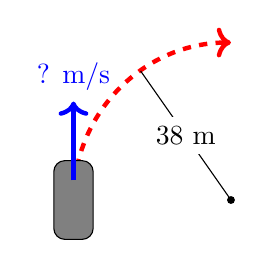
\begin{tikzpicture}
      \draw[dashed, ->, ultra thick, red] 
        (0,0) arc (180:90:2);
      \draw[rounded corners, fill=gray] 
        (-.25,-.5) rectangle ++ (0.5,1);
      \draw[] (2,0) -- ++ (125:2) 
        node[midway, fill=white] {38 m};
      \fill (2,0) circle (0.05);
      \draw[->,blue,ultra thick]
        (0,.25) -- ++ (0,1) node[above] {? m/s};
    \end{tikzpicture}
    \caption{(Original Diagram) A bird's-eye view of a car rounding a curve of radius 38~m.}
  \end{figure}


\myquestion (Giancolli P8)
How large must the coefficient of static friction be between the tires and the road if a car is to round a level curve of radius 125 m at a speed of 95 km/h (26.4~m/s)?
\answer{0.57}


\myquestion (Giancolli P15)
A coin is placed 13.0~cm from the axis of a rotating turntable of variable speed.
When the speed of the turntable is slowly increased, the coin remains fixed on the turntable until a rate of 38.0~rpm (revolutions per minute) is reached, at which point the coin slides off.
What is the coefficient of static friction between the coin and the turntable?
\answer{0.21}

\myquestion (OpenStax P32) \textbf{Unreasonable Results}
(a) Calculate the minimum coefficient of friction needed for a car to negotiate an unbanked 50.0 m radius curve at 30.0 m/s.
(b) What is unreasonable about the result?
(c) Which premises are unreasonable or inconsistent?
\answer{1.84}

\vs
\pagebreak
\uplevel{
  \subsection*{Conceptual Questions}
  }

\begin{enumerate}[resume*]
  \item Race car drivers routinely cut corners as shown in path \#2 in Figure~\ref{6.29}. Explain how this allows the curve to be taken at the greatest speed.
    \begin{figure}[ht]
      \centering
      \includegraphics[width=3.5cm]{6-29.jpg}
      \caption{(OpenStax Fig  6.29) Two paths around a race track curve are shown. Race car drivers will take the inside path (path \#2, called cutting the corner) whenever possible because it allows them to take the curve at the highest speed.}
      \label{6.29}
    \end{figure}

\end{enumerate}

\uplevel{
  \section*{Banked Turns}
  \subsection*{Problems}
  }

\myquestion \textbf{Bonus!} (OpenStax P25)
What is the ideal banking angle for a gentle turn of 1.20 km radius on a highway with a 105 km/h speed limit (about 65 mi/h), assuming everyone travels at the limit?
\answer{$4.14^\circ$}

\myquestion \textbf{Bonus!} (OpenStax P26)
What is the ideal speed to take a 100 m radius curve banked at a 20.0° angle?
\answer{18.9 m/s}

% \myquestion (OpenStax P27)
% (a) What is the radius of a bobsled turn banked at 75.0° and taken at 30.0 m/s, assuming it is ideally banked?
% (b) Calculate the centripetal acceleration.
% (c) Does this acceleration seem large to you?
% \answer{(a) 24.6 m; (b) 36.6 m/s$^2$; (c) $3.73 g$} 

\myquestion \textbf{Bonus!} (OpenStax P30)
If a car takes a banked curve at less than the ideal speed, friction is needed to keep it from sliding toward the inside of the curve (a real problem on icy mountain roads). (a) Calculate the ideal speed to take a 100 m radius curve banked at 15.0º. (b) What is the minimum coefficient of friction needed for a frightened driver to take the same curve at 20.0 km/h?
\answer{(a) 16.2 m/s; (b) 0.234}

\vs\pagebreak


\uplevel{
  \section*{Universal Gravitation}
  \subsection*{Problems}
  }

\begin{table}[h]
  \centering
  \begin{tabular}{lll}
    \hline\hline
    Earth: & Mass           & \SI{5.98e24}{kg} \\
           & Radius (mean)  & \SI{6.38e6}{m}  \\
    Moon:  & Mass           & \SI{7.35e22}{kg} \\
           & Radius (mean)  & \SI{1.74e6}{m}  \\
    Sun:   & Mass           & \SI{1.99e30}{kg} \\
           & Radius (mean)  & \SI{6.96e8}{m}  \\
    Mars:  & Mass           & \SI{6.42e23}{kg} \\
           & Radius (mean)  & \SI{3.38e6}{m}  \\
    Jupiter: & Mass         & \SI{1.90e27}{kg} \\
           & Radius (mean)  & \SI{6.99e7}{m}  \\
    \hline
    \multicolumn{2}{l}{Earth-Sun Distance (mean)} & 
                              \SI{1.496e11}{m} \\
    \multicolumn{2}{l}{Earth-Moon Distance (mean)} & 
                              \SI{3.84e8}{m}  \\
                              \hline\hline
  \end{tabular}
  \caption{Masses and sizes of various planets}
  \label{planets}
\end{table}

\myquestion (Original Question) \label{OPsat}
A satellite orbits the earth at a distance 1,120 km {\bf above the Earth's surface} (see Figure~\ref{satorbit}).  If the force of gravity acting on the satellite is \SI{2100}{\newton}, what is the mass of the satellite? (\emph{Hint:} think carefully about what the radius is and use the data in Table~\ref{planets} to help you.)
\answer{29.6 kg}

  \begin{figure}[h]
    \centering
    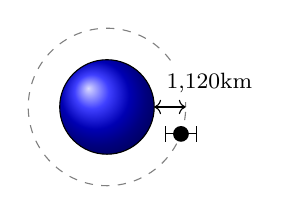
\begin{tikzpicture}
      \draw[shading=ball] (0,0) circle (.6);
      \draw[dashed,gray] (0,0) circle (1);
      \node[fill=white] at (1.3,.3)
        {\footnotesize \SI{1,120}{km}};
      \draw[<->] (.6,0) -- (1,0);
    
    
      \begin{scope}
        \fill (340:1) coordinate (satellite) 
          circle (0.1);
        \draw (satellite) 
          -- ++(.2,0) ++(0,.1) -- ++ (0,-.2);
        \draw (satellite) 
          -- ++(-.2,0) ++(0,.1) -- ++ (0,-.2);
      \end{scope}
    \end{tikzpicture}
    \caption{(Original Figure) For problem \ref{OPsat}}
    \label{satorbit}
  \end{figure}

\myquestion (OpenStax P39) 
(a) Calculate the magnitude of the gravitational force exerted on a 4.20-kg baby by a 100-kg father 0.200~m away at birth (he is assisting, so he is close to the child).
(b) Calculate the magnitude of the force on the baby due to Jupiter if it is at its closest distance to Earth, some \SI{6.29e11}{m} away. 
(c) How does the force of Jupiter on the baby compare to the force of the father on the baby? 
\answer{(a) \SI{7.01e-7}{N}; (b) \SI{1.35e-6}{N}; (c) $F_J=1.92 F_f$}

% \myquestion (OpenStax P34) 
% (a) Calculate the magnitude of the acceleration due to gravity on the surface of Earth due to the Moon.
% (b) Calculate the magnitude of the acceleration due to gravity at Earth due to the Sun.
% (c) Take the ratio of the Moon's acceleration to the Sun's and comment on why the tides are predominantly due to the Moon in spite of this number.
% \answer{(a) \SI{3.33e-5}{m/s^2}; (b) \SI{5.93e-3}{m/s^2}; (c) $a_S=178a_m$}

\myquestion (OpenStax P35) 
(a) What is the acceleration due to gravity on the surface of the Moon?
(b) On the surface of Mars?
\answer{(a) \SI{1.62}{m/s^2}; (b) \SI{3.75}{m/s^2}}

\myquestion (Giancolli P40)
You are explaining to friends why an astronaut feels weightless orbiting in the space shuttle, and they respond that they thought gravity was just a lot weaker up there.  Convince them that it isn't so by calculating how much weaker (in \%) gravity is 380 km above the Earth's surface.
\answer{$\SI{8.73}{m/s^2} = 89\% \text{ of } g_\text{surface}$}


\uplevel{
  \subsection*{Conceptual Questions}
  }

\begin{enumerate}[resume*]
  \item (Giancolli MC8) Which pulls harder gravitationally, the Earth on the Moon, or the Moon on the Earth? Which accelerates more?


\end{enumerate}


\uplevel{
  \section*{Satellites}
  \subsection*{Problems}
  }
  

\myquestion (Original Question)
  Use the data provided in Table~\ref{planets} to calculate (a) the force of gravity between the Earth and the Moon and (b) the tangential speed at which the Moon orbits the Earth.
  \answer{(a) \SI{1.99e20}{N}; (b) \SI{1020}{m/s}}

\myquestion (Giancolli P46)
Calculate the speed of a satellite moving in a stable circular orbit about the Earth at a height of 4800 km.  (Be careful to think about what the radius should be.)
\answer{\SI{5973}{m/s}}

\myquestion (Giancolli P52)
Determine the time it takes for a satellite to orbit the Earth in a circular near-Earth orbit. A ``near-Earth'' orbit is at a height above the surface of the Earth that is very small compared to the radius of the Earth.  [Hint: You may take the acceleration due to gravity as essentially the same as that on the surface.]. Does your result depend on the mass of the satellite?
\answer{\SI{1.41}{hr}}


\myquestion (OpenStax P43)
A geosynchronous Earth satellite is one that has an orbital period of precisely 1 day. Such orbits are useful for communication and weather observation because the satellite remains above the same point on Earth (provided it orbits in the equatorial plane in the same direction as Earth's rotation). Calculate the radius of such an orbit based on the data in Table~\ref{planets}.
\answer{\SI{4.23e7}{m}}

\end{questions}
\end{document}